\documentclass{article}
\usepackage{graphicx} % Required for inserting images
\usepackage[linesnumbered,ruled,vlined]{algorithm2e}
\usepackage{algpseudocode}

\title{Influence Maximization Algorithms}
\author{Aaron Frye and Ben Lenox}
\date{November 2024}

\begin{document}

% \includegraphics[scale=0.1]{diagram.jpg}

\maketitle

\section{Overview of Algorithm(s)}

The objective of this algorithm (these algorithms) is to find the node(s) with the maximal influence in a graph.  Influence can be anything that spreads along connections between nodes.  For example, the nodes could represent people and the edges could represent acquaintanceships and friendships.  The "influence" in question could be the spread of a rumor or other information. \\

Two algorithms were implemented to quantify the influence of each node in a graph.  One is a greedy influence maximization algorithm, and the other is an influence maximization algorithm based on the high degree heuristic.  Each algorithm calculates the influence of each node in a graph, and returns a map object (python's dict) that maps each node to the calculated influence value. \\

The greedy influence maximization algorithm is the more complex of the two.  This algorithm takes two parameters---trials, which represents the number of trials to use to calculate average influence (a greater number of trials will result in a slower but more accurate estimation of influence), as well as activation\_probability, which represents the probability of each node "activating" an adjacent node.  This algorithm essentially completes trials breadth-first searches for each node in the graph.  During each breadth-first search, only one node starts activated---the start node.  Each node adjacent to the start node has activation\_probability chance of being activated.  Each activated node will also be visited and will, in turn, have activation\_probability chance of activating its neighbors.  At the end of each breadth first search, the number of activated nodes (visited nodes) is counted.  The average number of nodes activated in any given trial is the calculated influence of a node. \\

The high-degree heuristic influence maximization algorithm calculates influence by looking at how many nodes a given node is adjacent to.  This is known as the degree of the node.  The degree of each node is the number calculated by this algorithm that represents the influence of each node.  This algorithm is generally understood to be less accurate than the greedy algorithm described above, but in many situations these algorithms will result in identical answers for the node with the maximum influence.  This algorithm is also much more efficient than the greedy algorithm, which is one reason this algorithm might be used despite being less accurate than the greedy algorithm.


\section{Pseudocode}

\begin{algorithm}[H]
\caption{$GreedyInfluenceMaximization(G, activationProbability, trials)$}
\KwIn{Graph $G$ -- an undirected graph, Float $activationProbability$ -- the probability that a node will spread its influence to a given adjacent node, Int $trials$ -- the number of trials to run for each node in calculating its influence}
\KwOut{A dictionary object containing nodes as keys with values being the calculated influence of each node}
$influenceAvg \gets $ new Dictionary\;
\ForEach{Node $n$ in $G.nodes$}{
	$influenceAvg[n] \gets 0$\;
}
\ForEach{Node $n$ in $G.nodes$}{
	\For{$\_ \gets 0$ \KwTo $trials$}{
		$Q \gets $ new Queue\;
		$Q.enqueue(n)$\;
		$visited \gets $ empty Set\;
		\While{$Q$ is not empty}{
			$curr \gets Q.dequeue()$\;
			add $curr$ to $visited$\;
			\ForEach{Node $n1$ adjacent to $n$ in $G$}{
				$rand \gets $ Random float between 0 and 1\;
				\If{$rand < activationProbability$ and $n1$ is not in $Q$ and $n1$ is not in $visited$}{
					$Q.enqueue(n1)$\;
				}
			}
		}
		$influenceAvg[n] \gets influenceAvg[n] + |visited|$\; 
	}
	$influenceAvg[n] \gets influenceAvg[n] / trials$\;
}
\Return{$influenceAvg$}\;
\end{algorithm}

\begin{algorithm}[H]
\caption{$HighDegreeHeuristicInfluenceMaximization(G)$}
\KwIn{Graph $G$ -- an undirected graph}
\KwOut{A dictionary object containing nodes as keys with values being the calculated influence of each node}
$influence \gets $ new Dictionary\;
\ForEach{Node $n$ in $G.nodes$}{
	$influence[n] \gets G.degree(n)$\;
}
\Return{$influence$}\;
\end{algorithm}

\section{Justification for Selection of Data Structures}

The implementation of the greedy algorithm uses three data structures other than NetworkX's graph.  First, a dictionary (hashmap) is used to store the influence values for each node.  This is done to provide constant time lookup and assignment of influence values during the calculation.  A queue is used for the breadth-first search that forms the basis of this algorithm.  The breadth first search adds activated nodes to the queue to be traversed and have a chance of activating its neighboring nodes.  A set is used to store the nodes that have been visited by the breadth-first search.  This is to make sure that no node is visited twice (as sets have a constant-time lookup of elements) and to count the number of visited nodes at the end of each breadth-first search. \\

The implementation of the high degree heuristic influence maximization algorithm simply uses a dictionary (hashmap).  The hashmap is used for constant assignment of influence value to each node and constant lookup when the dict is returned by the function.

\section{Intuition for Correctness}

These algorithms attempt to measure the influence of a node in a graph.  Let us think about this in an example scenario---the spread of a rumor in a city, town, community, etc.  One person will begin spreading the rumor and, depending on who the person is, it will reach a different number of people.  If the rumor reaches more people, then the person who started it has more "influence." \\

The greedy algorithm attempts to measure this influence using a random chance of node activation.  In our implementation of the greedy algorithm, the person who started the rumor will have a 20\% chance of spreading the rumor to each of their friends.  In turn, each friend who hears the rumor will also have a 20\% chance of spreading it to each of their friends.  Once all people and friendships have been exhausted, the number of people to whom the rumor was spread will be counted.  If this process is done many times, the average number of people who hear the rumor is the "influence" of the person who started the rumor.  This process is done with each node in the graph to find their influence.  We can see here how the more influential people (nodes) will have a greater influence value. \\

The high degree heuristic algorithm attempts to measure influence by asking how many friends a person has (edges connected to a given node).  Generally, the people with more friends will spread the rumor further, because the rumor has a larger base audience.  This will not always be true, though, which is why this algorithm is regarded as less accurate than the greedy algorithm.  Below is a good example of when these algorithms will give different results.  While the node in the upper part of the graph (selected by the high degree heuristic algorithm) has more edges, the node in the lower part of the graph (selected by the greedy algorithm) clearly has more influence on the rest of the graph because it is more well connected to a greater number of nodes.

\begin{center}
\makebox[\textwidth]{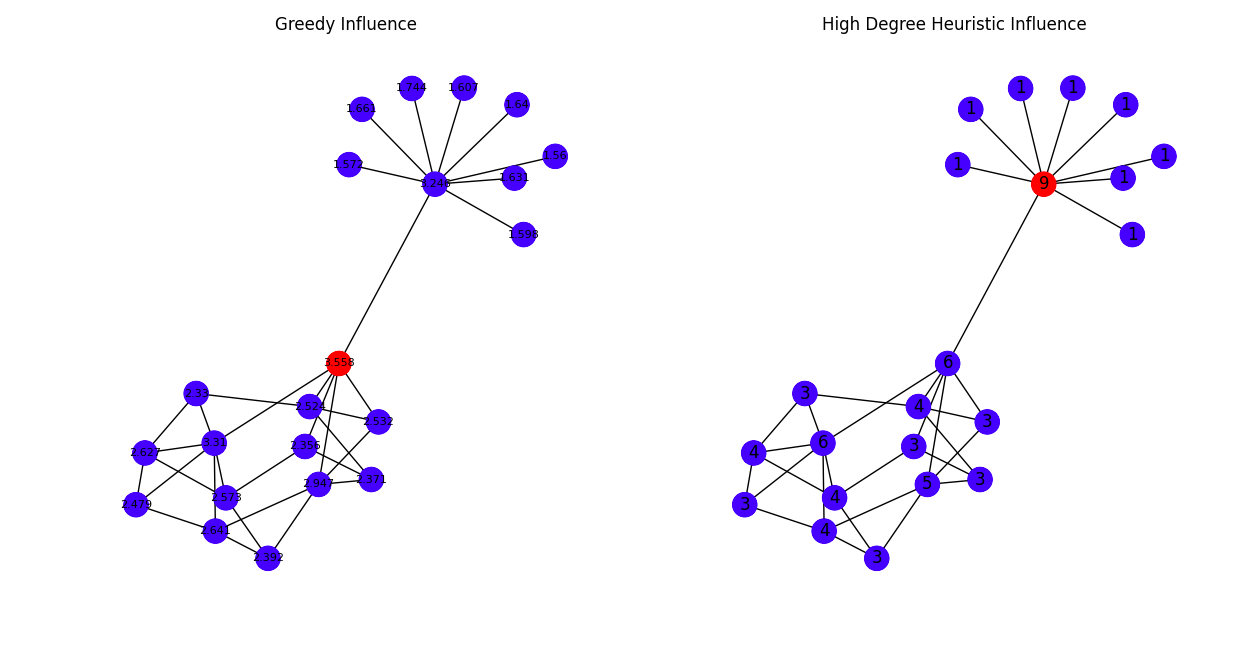
\includegraphics[scale=0.45]{test19.png}}
\end{center}


\section{Time Complexity Analysis}

The greedy influence maximization algorithm has one main loop that executes over each node in the input graph.  This loop runs a breadth-first search trials times, where trials is the input that specifies how many times to run a trial to determine the average influence of each node.  Breadth-first search runs in $\Theta(n + m)$ time, because each node and each edge is traversed exactly once.  For this implementation of breadth-first search, it is likely that not every node in the graph will be traversed because there is a random probability of node activation.  Still, there is the potential for every breadth-first search that each node and each edge is visited exactly once in the worst case.  This means that the breadth-first search in our implementation also runs in $\Theta(n + m)$ time.  Breadth-first search is run once for each trial for each node in the graph. This means that the total time complexity of the greedy influence maximization algorithm is $\Theta(nt(n + m))$ where t is the number of trials that are run for each node, n is the number of nodes in the graph, and m is the number of edges in the graph. \\

The high-degree heuristic algorithm runs in $\Theta(n)$ time.  Each node is looped over, and the degree of the node is assigned to the value of a dictionary keyed on nodes in the graph.

\section{Space Complexity Analysis}

The greedy influence maximization algorithm has a space complexity of $\Theta(n)$.  The algorithm keeps track of a dictionary that stores n keys representing nodes in the input graph, and n values representing the influence of the nodes in the graph.  In each iteration of the main loop in the algorithm, a queue and a set are formed for a breadth-first traversal of the input graph.  The queue and the set can have as many as n nodes.  These data structures are not retained between iterations, so python's garbage collector can free the space assigned to them.  Therefore, the space complexity of this algorithm is $\Theta(n)$. \\

The high-degree heuristic algorithm has a space complexity of $\Theta(n)$.  Only one data structure is used for this algorithm---a dictionary that maps nodes to their influence value.  This dictionary contains n keys and n values, so its space usage is proportional to n.  This algorithm therefore has a space complexity of $\Theta(n)$.


\section{Python Code}

\begin{verbatim}
import networkx as nx
import matplotlib.pyplot as plt
from collections import deque
from random import random
from itertools import combinations

def greedy_influence_maximization(G, activation_probability=0.2, trials=1000):
    nodes = G.nodes
    adj = G.adj
    influence_avg = {n: 0 for n in nodes}
    for n in nodes:
        for _ in range(trials):
            q = deque()
            q.append(n)
            visited = set()
            while q:
                curr = q.popleft()
                visited.add(curr)
                for n1 in adj[curr]:
                    if random() < activation_probability and n1 not in q and n1 not in visited:
                        q.append(n1)
            influence_avg[n] += len(visited)
        influence_avg[n] /= trials
    return influence_avg

def high_degree_heuristic_influence_maximization(G):
    nodes = G.nodes
    influence = {n: G.degree(n) for n in nodes}
    return influence

def test(G):
    G1 = G.copy()
    greedy = greedy_influence_maximization(G)
    greedy_max = max(greedy.values())

    high_degree = high_degree_heuristic_influence_maximization(G)
    high_degree_max = max(high_degree.values())

    nx.set_node_attributes(G1, greedy, "greedy_influence")
    nx.set_node_attributes(G1, high_degree, "high_degree_influence")

    fig, axes = plt.subplots(1, 2)
    pos = nx.spring_layout(G1, k=0.05)


    axes[0].set_title("Greedy Influence")
    axes[1].set_title("High Degree Heuristic Influence")

    nx.draw(G1, pos, ax=axes[0], node_color=["red" if greedy[node] == greedy_max else "blue" for node in G.nodes])
    nx.draw(G1, pos, ax=axes[1], node_color=["red" if high_degree[node] == high_degree_max else "blue" for node in G.nodes])
    # nx.draw(G1, pos, with_labels=True)

    nx.draw_networkx_labels(G1, pos, ax=axes[0], labels = greedy, font_size=8)
    nx.draw_networkx_labels(G1, pos, ax=axes[1], labels = high_degree)

    plt.show()

# Intuition for differences between algorithms
G1 = nx.Graph([(1, 2), (1, 3), (1, 4), (1, 5), (1, 6), (1, 7), (1, 8), (1, 9), (1, 10), (10, 11), (10, 13), (16, 17), (15, 17), (13, 11), (10, 14), (10, 21), (14, 15), (14, 16), (14, 17), (14, 18), (18, 17), (19, 18), (20, 19), (20, 21), (11, 21), (12, 21), (22, 12), (21, 22), (15, 13), (10, 19), (12, 14), (22, 18), (16, 12), (20, 13)])

# Test 1
# G1 = nx.connected_watts_strogatz_graph(100, 5, 0.2)
# Test 2
# G1 = nx.fast_gnp_random_graph(20, 0.2)
# isolated_nodes = list(nx.isolates(G1))
# Test 3
# G1.remove_nodes_from(isolated_nodes)
# Test 4
# G1 = nx.generators.community.stochastic_block_model([10, 25, 13], [[0.8, 0.1, 0.1], [0.1, 0.8, 0.1], [0.1, 0.1, 0.8]])
# Test 5
# G1 = nx.gaussian_random_partition_graph(70, 15, 5, 0.4, 0.05)
# Test 6
# G1 = nx.Graph()
# G1.add_nodes_from([*range(1,11)])
# Test 7
# G1 = nx.Graph([*combinations(range(1,11), 2)])
# Test 8
# G1 = nx.Graph([*combinations(range(1,6), 2)] + [*combinations(range(6,11), 2)] + [*combinations(range(11,16), 2)])
test(G1)

\end{verbatim}

\section{Tests}

The use case of this algorithm is to detect influential nodes in graphs.  This type of algorithm is often used in social networks with the connections being relations among people, but it does not have to be.  Influence can be measured among nodes in graphs where there is no community structure as well.  Influence maximization algorithms can also be a measure of centrality.  For example, in a graph of cities and flight paths, nodes with high influence would likely be more heavily trafficked.  For these reasons, the main test used for these algorithms will use a variety of random graph generation techniques, including with and without community structures. \\

A successful test case would show a highlighted node (a node with maximal influence) that appears central to the graph.  There should be a large number of paths between the chosen node and any other node. \\

\subsection{Test 1}
    \begin{center}
        \makebox[\textwidth]{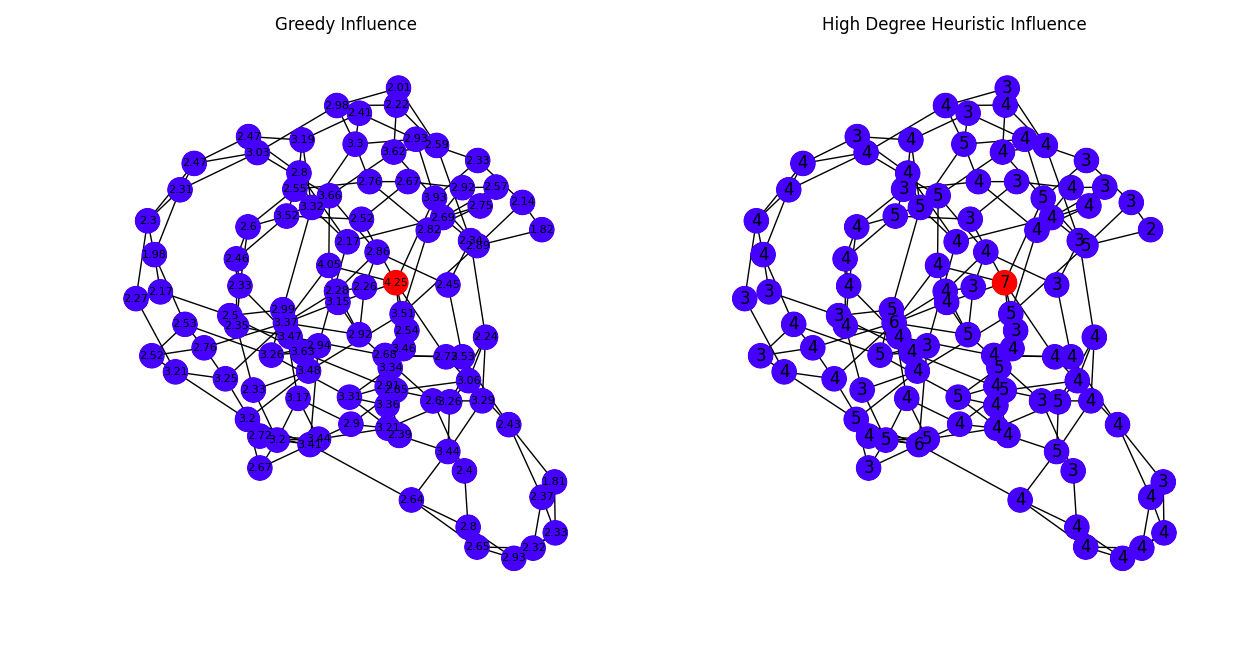
\includegraphics[scale=0.45]{test11.png}}
    \end{center}
\subsection{Test 2}
    \begin{center}
        \makebox[\textwidth]{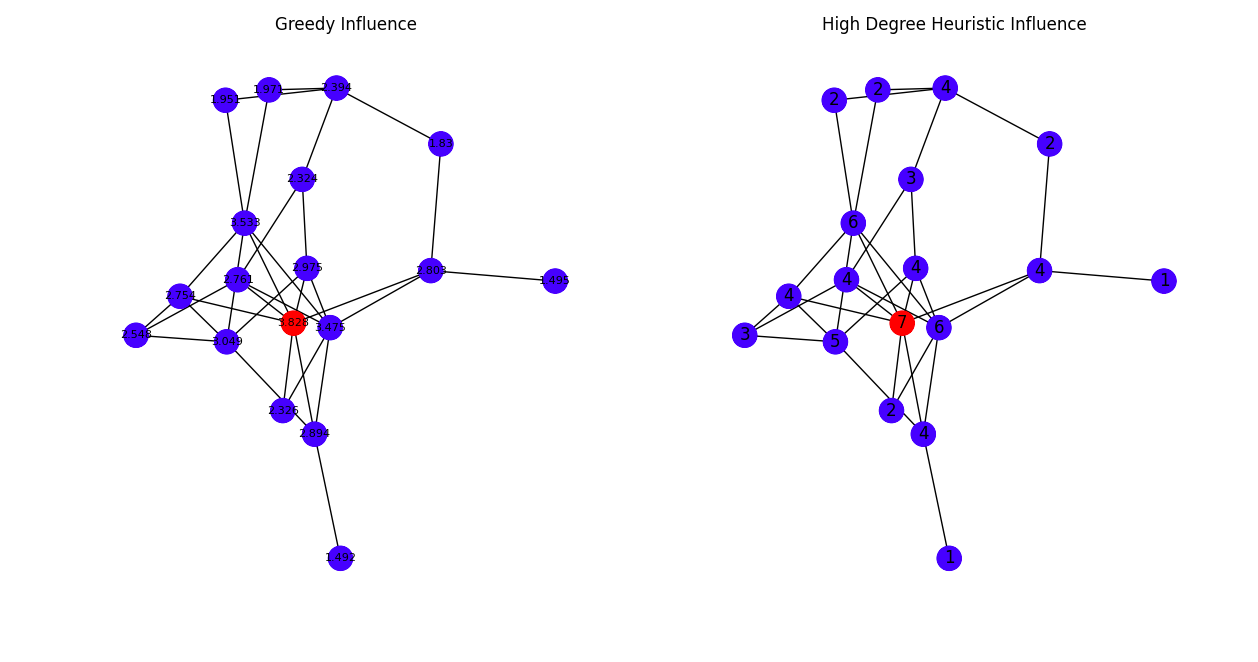
\includegraphics[scale=0.45]{test12.png}}
    \end{center}
\subsection{Test 3}
    \begin{center}
        \makebox[\textwidth]{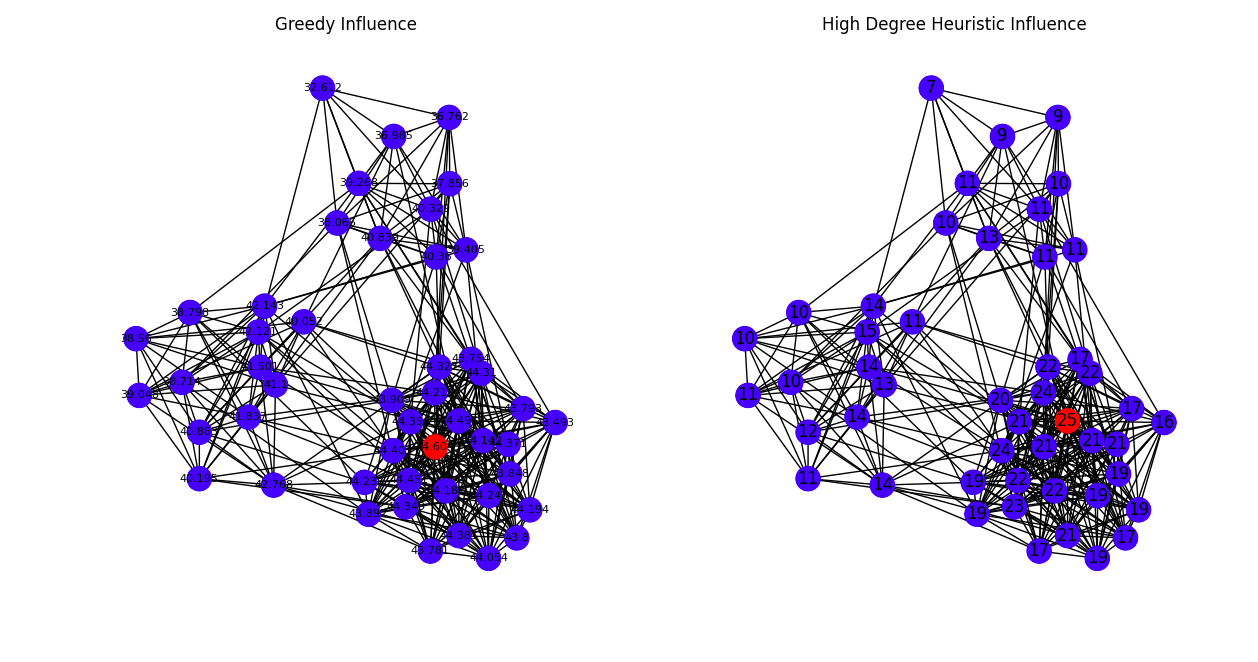
\includegraphics[scale=0.45]{test13.png}}
    \end{center}
\subsection{Test 4}
    \begin{center}
        \makebox[\textwidth]{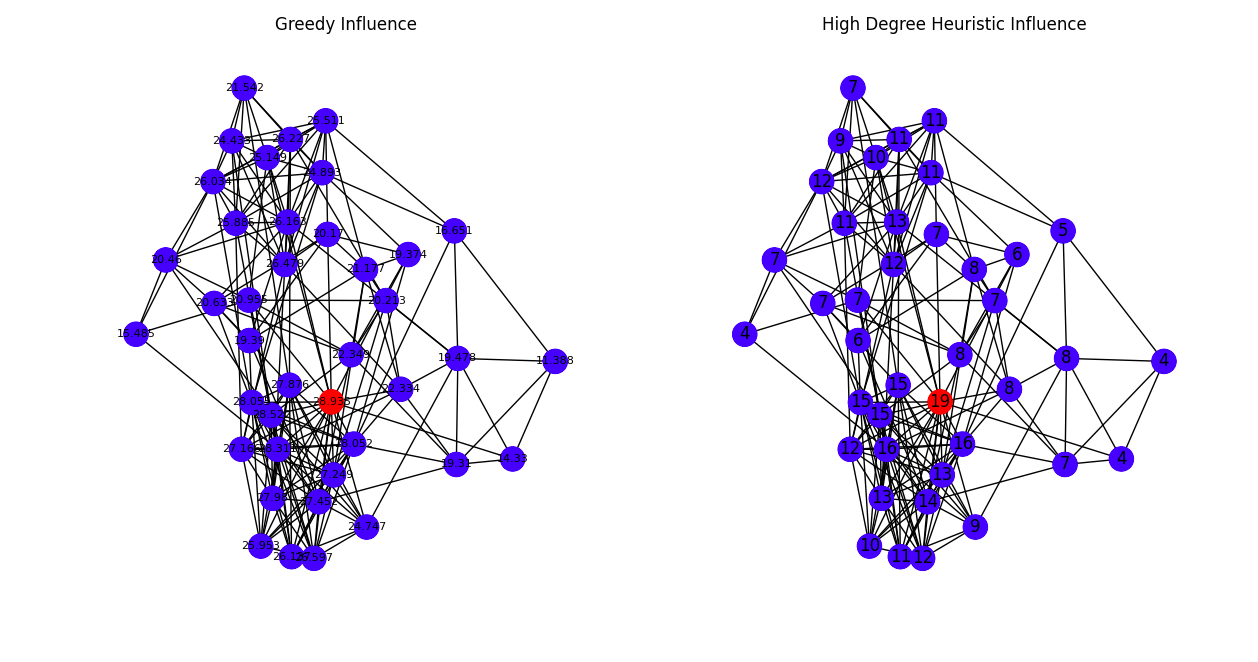
\includegraphics[scale=0.45]{test14.png}}
    \end{center}
\subsection{Test 5}
    \begin{center}
        \makebox[\textwidth]{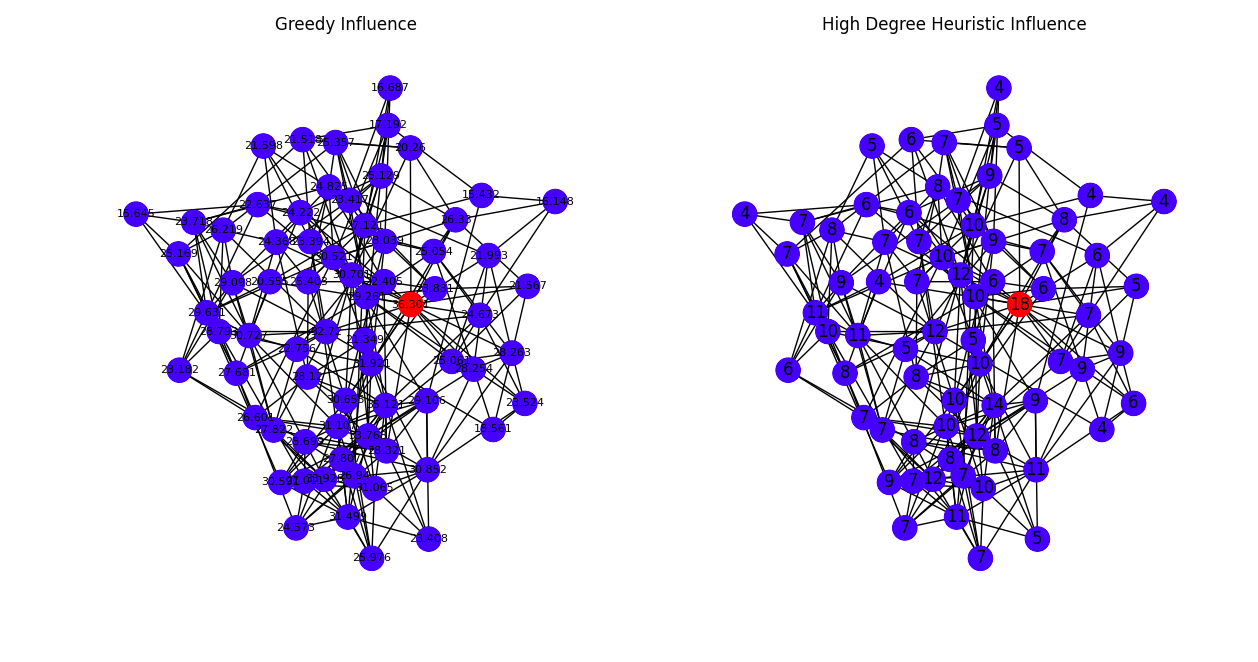
\includegraphics[scale=0.45]{test15.png}}
    \end{center}

We can see that these two algorithms often pick out nodes that are visually more "central" to the graph.  These nodes have the ability to influence other nodes relatively easily given their centrality---they have a large number of paths to many nodes in the graph.  We can also see that oftentimes, the node with the highest degree will be the one with the highest influence using the greedy method.  This is expected---a node with a high degree will be able to reach many other nodes with a large number of paths. \\ 

Edge cases for these algorithms would be cases where each node has the same influence or each node has no influence.  The greedy algorithm would be expected to choose a random node in this case, because the average is generated via random chances of node activation.  In the case of each node having no edges, the greedy algorithm should choose all nodes, because the influence will be exactly 1 (only the start node is activated).  The high degree heuristic should generate all nodes being equal in these cases, because each node would have exactly equal degree. \\

\subsection{Test 6}
    \begin{center}
        \makebox[\textwidth]{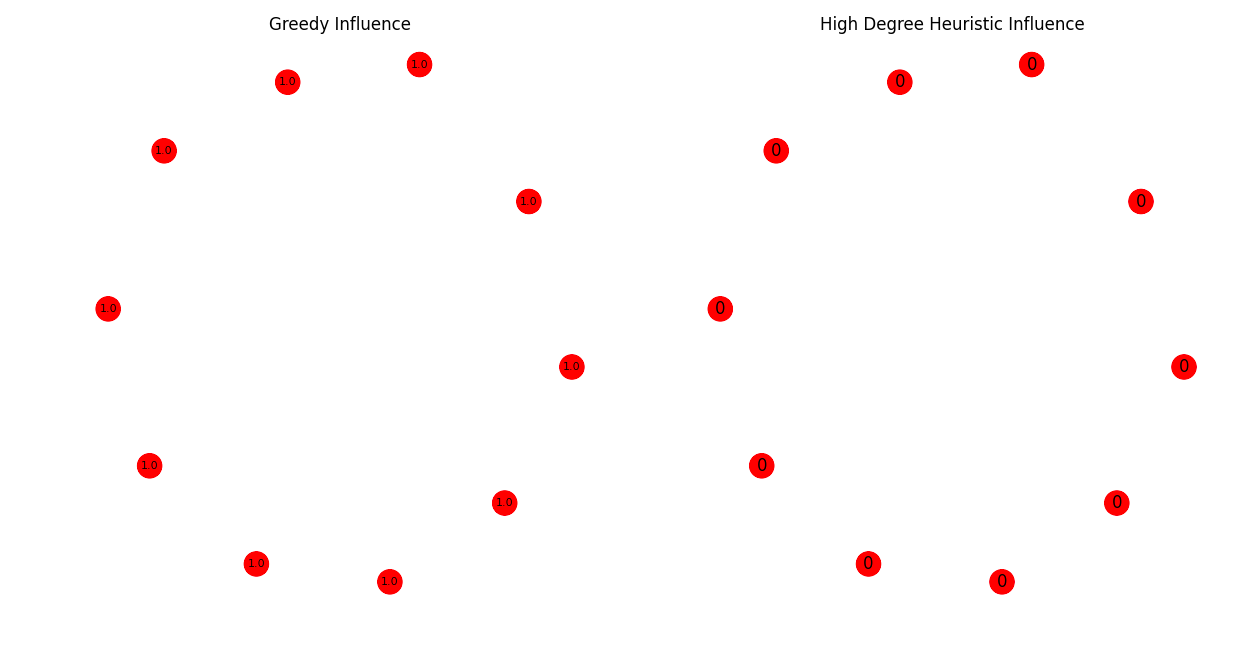
\includegraphics[scale=0.45]{test16.png}}
    \end{center}
\subsection{Test 7}
    \begin{center}
        \makebox[\textwidth]{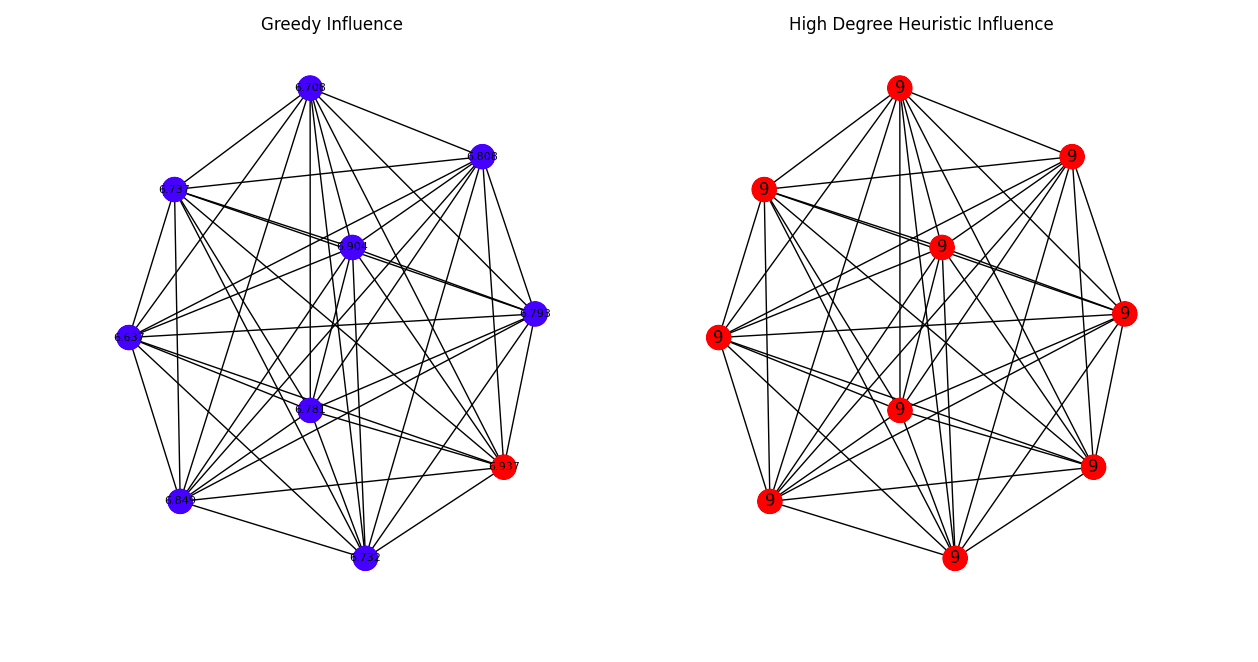
\includegraphics[scale=0.45]{test17.png}}
    \end{center}
\subsection{Test 8}
    \begin{center}
        \makebox[\textwidth]{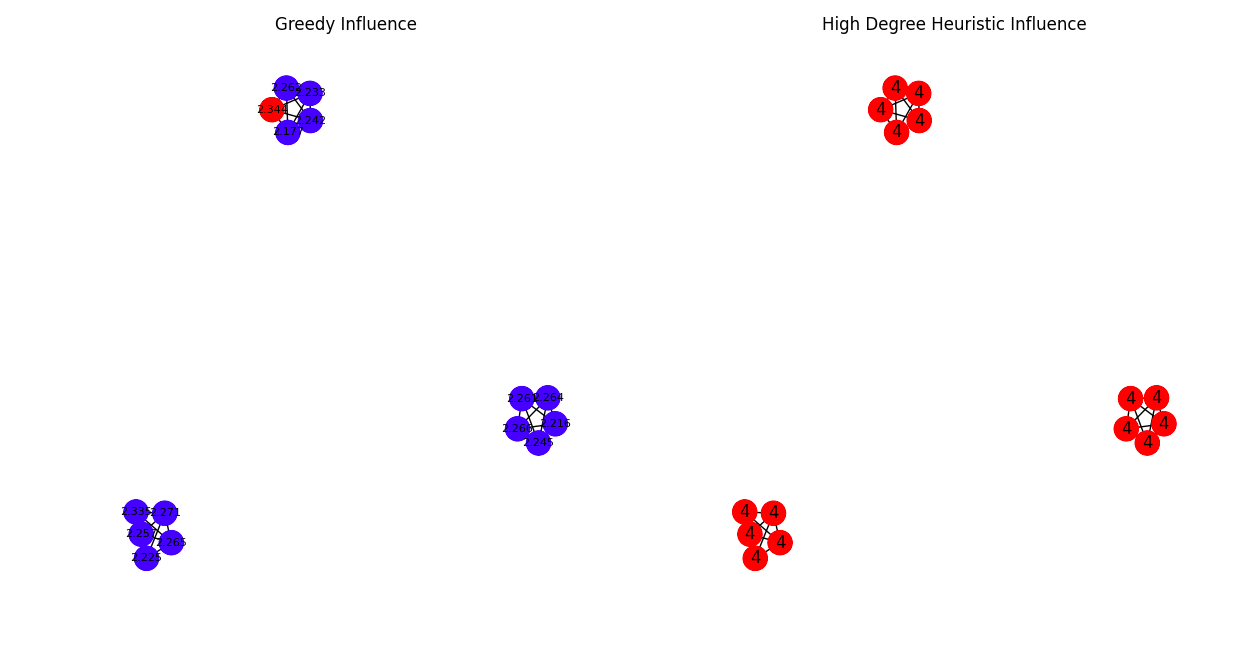
\includegraphics[scale=0.45]{test18.png}}
    \end{center}

These edge test cases do have the expected output.  For the graph with no edges, these algorithms show each node having the minimum possible influence---1 in the case of the greedy algorithms and 0 in the case of the high degree heuristic algorithm.  In the test cases where each node has an equal degree, the greedy algorithm shows that the influence of each node is very close to the influence of the other nodes.  This is consistent with the random approximation of influence the algorithm uses.  The high degree heuristic algorithm shows each node has equal influence (as they each have equal degree).

\end{document}
